\documentclass[12pt]{article}

\usepackage[a4paper]{geometry} %page size
\usepackage{parskip} %no paragraph indentation
\usepackage{fancyhdr} %fancy stuff in page header
\pagestyle{fancy} 

\usepackage[utf8]{inputenc} %encoding
\usepackage[danish]{babel} %danish letters

\usepackage{graphicx} %import pictures

\usepackage{amsmath, amssymb, amsfonts, amsthm, mathtools} %doing math
\usepackage{algorithmicx, algpseudocode} %doing pseudocode,

\fancyhead{}
\lhead{Machine Learning: Home Assignment 1}
\rhead{Asger Andersen}

%End of preamble
%*******************************************************************************

\begin{document}

\section{Vectors and Matrices}

I have chosen not to answer this optional question.

\section{Derivatives}

I have chosen not to answer this optional question.

\section{Probability Theory: Sample Space}

I have chosen not to answer this optional question.

\section{Probability Theory: Properties of Expectation}

Let $X$ and $Y$ be two discrete random variables taking values in $\mathcal{X}$ and $\mathcal{Y}$, respectively.

\textbf{Question 1:} Let me now proof that
\begin{align}
\mathbb{E}[X + Y] = \mathbb{E}[X] + \mathbb{E}[Y]
\end{align}

Let $p_{X,Y}$ be the joint distribution of $X$ and $Y$, and let $p_X$ and $p_Y$ be the marginal distributions of $X$ and $Y$, respectively. By definition of the marginalization of a discrete random variable, we know for all $x \in \mathcal{X}$ and $y \in \mathcal{Y}$ that
\begin{align}
\sum_{y \in \mathcal{Y}} p_{X,Y}(x,y) = p_X(x)
\end{align}
and
\begin{align}
\sum_{x \in \mathcal{X}} p_{X,Y}(x,y) = p_Y(y)
\end{align}
From these statements and the definition of the expectation of a discrete random variable, it follows that 
\begin{align}
\mathbb{E}[X + Y] = \sum_{(x,y) \in \mathcal{X}\times \mathcal{Y}} p_{X,Y}(x,y)(x+y) = \\ 
\left( \sum_{(x,y) \in \mathcal{X}\times \mathcal{Y}} p_{X,Y}(x,y)x \right) + \left( \sum_{(x,y) \in \mathcal{X}\times \mathcal{Y}}p_{X,Y}(x,y)y \right) = \\ 
\left( \sum_{x \in \mathcal{X}} x \sum_{y \in \mathcal{Y}} p_{X,Y}(x,y) \right) + \left( \sum_{y \in \mathcal{Y}} y \sum_{x \in \mathcal{X}} p_{X,Y}(x,y) \right) = \\ 
\left( \sum_{x \in \mathcal{X}} x p_X(x) \right) + \left( \sum_{y \in \mathcal{Y}} y p_Y(y) \right) = \mathbb{E}[X] + \mathbb{E}[Y]
\end{align}
which proofs the statement on line (1).

\textbf{Question 2:} Assume now that $X$ and $Y$ are independent. Let me now proof that
\begin{align}
\mathbb{E}[XY] = \mathbb{E}[X]\mathbb{E}[Y]
\end{align}

By definition of indepence of random variables, we now know for all $x \in \mathcal{X}$ and $y \in \mathcal{Y}$ that 
\begin{align}
p_{X,Y}(x,y) = p_X(x)p_Y(y)
\end{align}
From these statements and the definition of the expectation of a discrete random variable, it follows that 
\begin{align}
\mathbb{E}[XY] = \\ \sum_{(x,y) \in \mathcal{X}\times \mathcal{Y}} p_{X,Y}(x,y)(xy) = \\
\sum_{(x,y) \in \mathcal{X}\times \mathcal{Y}} p_X(x)p_Y(y)xy = \\ 
\sum_{x \in \mathcal{X}} p_X(x)x \sum_{y \in \mathcal{Y}} p_Y(y)y = \\
\mathbb{E}[X]\mathbb{E}[Y]
\end{align}
which proofs the statement on line (8).

\textbf{Question 3:} Now throw away the assumption that $X$ and $Y$ are independent, and assume that $\mathcal{X} = \{x_1, x_2\}$ and $\mathcal{Y} = \{y_1, y_2\}$. Then this table would provide one option for a valid definition of the joint probability distribution $p_{X,Y}$:
\begin{center}
\begin{tabular}{lllll}
                           & $x_1$                      & $x_2$                      &     &  \\ \cline{2-3}
\multicolumn{1}{l|}{$y_1$} & \multicolumn{1}{l|}{0.001} & \multicolumn{1}{l|}{0.199} & 0.2 &  \\ \cline{2-3}
\multicolumn{1}{l|}{$y_2$} & \multicolumn{1}{l|}{0.499} & \multicolumn{1}{l|}{0.301} & 0.8 &  \\ \cline{2-3}
                           & 0.5                        & 0.5                        &     & 
\end{tabular}
\end{center}

We see that with this definition of $p_{X,Y}$, then $X$ and $Y$ are not independent, since we for instance have that 
\begin{align}
p_{X_Y}(x_1,y_1)=0.001 \neq 0.1 = p_X(x_1)p_Y(y_1)
\end{align}
We therefore might have - depending on the values of $x_1, x_2, y_1$ and $y_2$ - that line (8) does not hold for $X$ and $Y$. If we for instance set $x_1 = 1000, x_2 = -1, y_1 = 1000$ and $y_2 = -1$, then we have that 
\begin{align}
\mathbb{E}[XY] = 0.001 \cdot 1000000 - 0.199 \cdot 1000 - 0.499 \cdot 1000 + 0.301 \cdot 1 = 302.301
\end{align}
and 
\begin{align}
\mathbb{E}[X]\mathbb{E}[Y] = 0.1 \cdot 1000000 - 0.1 \cdot 1000 - 0.4 \cdot 1000 + 0.4 \cdot 1 = 99500.4
\end{align}
In this case, we clearly see that $\mathbb{E}[XY] \neq \mathbb{E}[X]\mathbb{E}[Y]$.

\textbf{Question 4:} Now go back to the definition of $X$ as an arbitrary discrete, random variable. Let me now proof that 
\begin{align}
\mathbb{E}[\mathbb{E}[X]] =\mathbb{E}[X]
\end{align}
Let $\mathbb{E}[X]$ be denoted $a$. Note that $a$ is just some real number. Since $p_X$ is a probability distribution, we know that 
\begin{align}
 \sum_{x\in \mathcal{X}}p_X(x) = 1
\end{align}

We now have that
\begin{align}
\mathbb{E}[\mathbb{E}[X]] = \mathbb{E}[a] = \sum_{x\in \mathcal{X}} p_X(x) a = a \sum_{x\in \mathcal{X}} p_X(x) = a = \mathbb{E}[X]
\end{align}
which proofs the statement on line (18).

\textbf{Question 5:} Let me now proof that 
\begin{align}
\mathbb{V}[X] = \mathbb{E}[(X - \mathbb{E}[X])^2] = \mathbb{E}[X^2] - (\mathbb{E}[X])^2
\end{align}
This we can proof by simply completing the square, and then using our results from question 1 and 3:
\begin{align}
\mathbb{E}[(X - \mathbb{E}[X])^2] = \\
\mathbb{E}[(X^2 + (\mathbb{E}[X])^2 - 2X\mathbb{E}[X]] = \\ 
\mathbb{E}[X^2] + \mathbb{E}[(\mathbb{E}[X])^2] - \mathbb{E}[2X\mathbb{E}[X]] = \\ 
\mathbb{E}[X^2] + (\mathbb{E}[X])^2 - 2 \mathbb{E}[X]\mathbb{E}[\mathbb{E}[X]] = \\ 
\mathbb{E}[X^2] + (\mathbb{E}[X])^2 - 2 \mathbb{E}[X]\mathbb{E}[X] = \\ 
\mathbb{E}[X^2] + (\mathbb{E}[X])^2 - 2 (\mathbb{E}[X])^2 = \\ 
\mathbb{E}[X^2] - (\mathbb{E}[X])^2
\end{align}

\section{Probability Theory: Complements of Events}

\textbf{Question 1:} Let $\mathbb{P}$ be any probability distribution over some sample space $\Omega$, and let $A \subset \Omega$ be some event. By definition of the complement event $\overline{A}$, we know that 
\begin{align}
A \cup \overline{A} = \Omega 
\end{align}
From the axioms of probability, we also know that
\begin{align}
\mathbb{P}(\Omega) = 1
\end{align}
and that
\begin{align}
\mathbb{P}(A \cup \overline{A}) = \mathbb{P}(A) + \mathbb{P}(\overline{A})
\end{align}
since $A$ and $\overline{A}$ are mutually exclusive.
From these three statements it follows that
\begin{align}
1 = \mathbb{P}(\Omega) = \mathbb{P}(A \cup \overline{A}) = \mathbb{P}(A) + \mathbb{P}(\overline{A})
\end{align}
from which it follows that
\begin{align}
\mathbb{P}(A) = 1 - \mathbb{P}(A)
\end{align}
which is what I was asked to proof.

\textbf{Question 2:} We flip a fair coin 10 times. What is probability that we observe at least one tail? The complement event of observing at least one tail is only observing heads on all 10 flips. The probability of observing a head on single flip is one half, and since all the flips are independent the probability of observing 10 heads is 
\begin{align}
\left(\frac{1}{2}\right)^{10} \approx 0.000977 
\end{align}
The probability of oberserving at least one tail on 10 flips is therefore
\begin{align}
1 - \left(\frac{1}{2}\right)^{10} \approx  1 - 0.000977 = 0.999023
\end{align}
What is the probability that we observe at least two tails. The complement event is that observe zero or only one tail. From the cumulative binomial distribution we get that the probability of this complement event is approximately 0.010742. Therefore, the probability of observing at least two tails is approximately
\begin{align}
1 - 0.010742 = 0.989258
\end{align} 

\section{Digit Classification with Nearest Neighbours}

This is some section!

\section{Linear Regression}

Since source code is listed as one of the deliverables in the assignment text, I show you here the source code of my python implementation of the linear regression algorithm, as it is described in the Data Mining Lecture Notes by Christian Igel: 

\begin{verbatim}
import scipy as scp

def linear_regression(x, y) :
    
    if (x.ndim == 1) : x = scp.matrix(x).T
    else : x = scp.matrix(x)
    y = scp.matrix(y).T
    
    
    ones_column = scp.tile([1], (x.shape[0], 1))
    x = scp.concatenate((x, ones_column), axis=1)
    
    w = (((((x.T * x).I) * x.T))* y ).A
    
    b = w[-1,0]
    w = w[0:-1].flatten()
    
    predict = lambda new : scp.dot(w, new) + b
    
    return {'hyp' : predict, 
            'est_params' : {'weigths': w, 
                            'bias': b}}
\end{verbatim}

The implementation uses the scipy library to take care of the linear algebra. As input it takes a scipy 2d-array as x (the sample) and a scipy 1d-array as y (the labels). As output it gives a dictionary containing 1) the linear model, which minimizes the squared error between the models predictions and the actual labels, and 2) the weight and bias parameters of the model. When I run this implementation on the Danwood data, I get the weight parameter 9.489 and the bias parameter -10.427. This means that my resulting model $h$ looks like:

\begin{align}
h(x) = 9.489x - 10.427
\end{align}

When I plot this model against the actual data, I get the following plot:

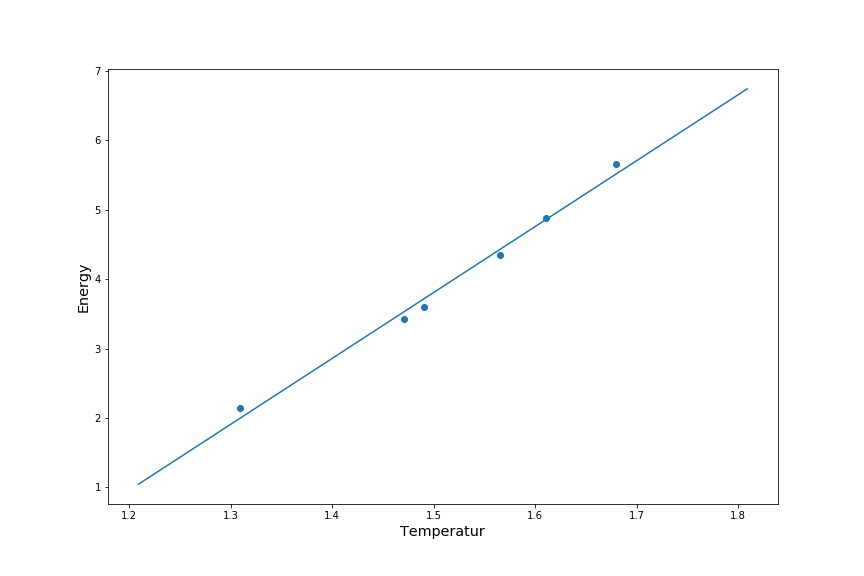
\includegraphics[scale = 0.45]{linear_regression/reg_plot_1.jpg}

The mean squared error of this model is 0.012. The variance of y (the energy measurements) is 1.269. The quotient of the mean squared error of the model over variance of y is 0.009. There are multiple ways to interpret this number in the context of linear regression. One way is to say that it is a measure of the how much smaller the error is, when we choose all linear functions as our model space instead of just constant functions (since the mean of y would be the squared error minimizer in the space of all constant models, and therefore the variance of y would be the mse of the chosen model in this space). In this interpretation it becomes clear that the quotient cannot be larger than 1, since the constant models are a subclass of the linear models. This also shows us that just because the quotient is a little smaller than 1, this does not mean that we have made a good decision by choosing all linear functions as our model space. It is not good to choose a much more complex model space, if we just get a small error reduction from it (especially in our current set up of linear regression, where we have no distinction between training and test set!). However, with the Danwood data we get approximately a reduction of factor 100, so it might be a good idea to model the data with linear instead of just constant functions. This is also quite obvious from just looking at the data (the orange line is the best constant model):

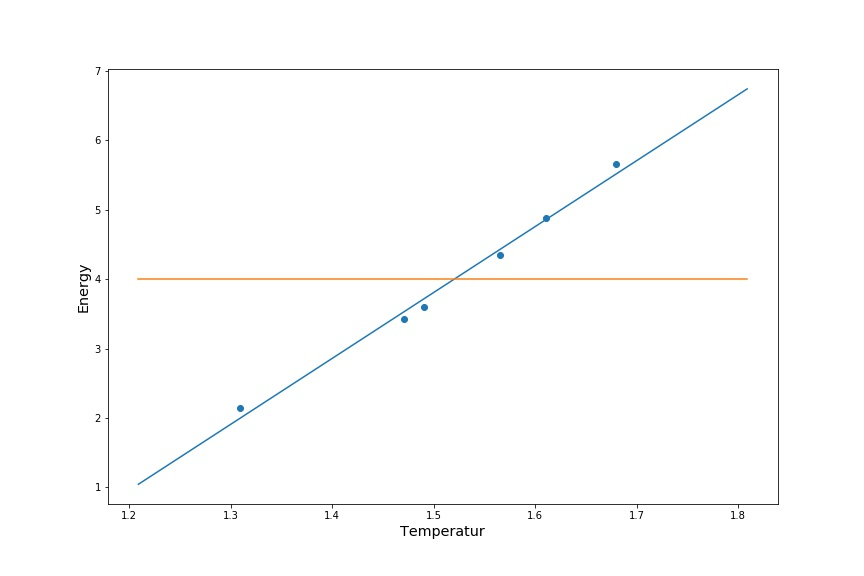
\includegraphics[scale = 0.45]{linear_regression/reg_plot_2.jpg}




\end{document}